\documentclass[tikz]{standalone}
% \usepackage{tikz} % already loaded by the documentclass
\usepackage{pgfplots}\usepackage{amssymb}\pgfplotsset{compat=1.18}

\begin{document}
%%| filename: exp-map
%%| additionalPackages: \usepackage{pgfplots}\usepackage{amssymb}\pgfplotsset{compat=1.18}

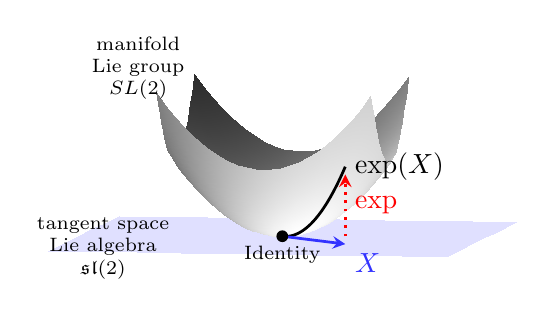
\begin{tikzpicture}[>=stealth]
\begin{axis}[
    hide axis,
    view={10}{5},
    xmin=-1.5, xmax=1.5,
    ymin=-1.5, ymax=1.5,
    zmin=-1, zmax=1.5,
    axis equal image,
    z buffer=sort
]
    \addplot3[
        surf,
        domain=-1.3:1.3, domain y=-1.3:1.3,
        samples=10,
        colormap={blueplane}{color=(blue!60) color=(blue!60)},
        fill opacity=0.2, shader=interp,
        faceted color=none, draw=none
    ] (x, y, 0);
    
% Light source position (change these to move the light)
\def\Lx{-1}
\def\Ly{1}
\def\Lz{3}
\pgfmathsetmacro{\Lnorm}{sqrt((\Lx)^2 + (\Ly)^2 + (\Lz)^2)}

\addplot3[
    surf,
    domain=-0.7:0.7, domain y=-0.7:0.7,
    samples=25,
    point meta={
        max(0, (-2*x*(\Lx) - 2*y*(\Ly) + (\Lz))
               / sqrt(4*x^2 + 4*y^2 + 1) / \Lnorm)
    },
    colormap={shade}{color=(black!85) color=(white)},
    shader=interp,
    faceted color=none,
    draw=none,
] {x^2 + y^2};
% \addplot3[
%         surf,
%         domain=-0.7:0.7, domain y=-0.7:0.7,
%         samples=20,
%         colormap={pureblack}{color=(gray) color=(gray)},
%         fill=none, fill opacity=0.0,
%         faceted color=black!10, thin,
%         shader=flat corner
%     ] {(x^2 + y^2)};


    \addplot3[color=black, line width=1.0pt, domain=0:0.5, samples=30]
        (x, -x, {x^2 + x^2});

    \draw[->, blue!80, line width=1.0pt]
        (axis cs:0,0,0) -- (axis cs:0.5,-0.5,0);

    % red arrow now points UP: plane -> manifold (the exp map)
    \draw[->, red, line width=1.0pt, dotted]
        (axis cs:0.5,-0.5,0.05) -- (axis cs:0.5,-0.5,0.45);

    \node[circle, fill=black, inner sep=1.5pt] at (axis cs:0,0,0) {};

    % --- TEXT LABELS ---
    \node[anchor=east, align=center, font=\scriptsize] at (axis cs:-0.5,-1,0)
        {tangent space\\Lie algebra\\$\mathfrak{sl}(2)$};

    \node[anchor=south east, align=center, font=\scriptsize] at (axis cs:-0.7,0.7,0.75)
        {manifold\\Lie group\\$SL(2)$};

    \node[anchor=north, font=\scriptsize] at (axis cs:0,0,0) {Identity};

    \node[anchor=north west, blue!80] at (axis cs:0.5,-0.5,0) {$X$};
    \node[anchor=west] at (axis cs:0.5,-0.5,0.5) {$\exp(X)$};
    \node[anchor=west, red] at (axis cs:0.5,-0.5,0.25) {$\exp$};
\end{axis}
\end{tikzpicture}
\end{document}
      